\documentclass[12pt, hidelinks]{article}
\usepackage[a4paper, margin=1in]{geometry} % Set 1-inch border
\usepackage[backend=biber, citestyle=ieee]{biblatex}
\usepackage{setspace}
\usepackage{acronym}
\usepackage{float}
\usepackage{hyperref}
\usepackage{setspace}
\usepackage{lipsum} % Dummy text
\usepackage{multirow} % Table
\usepackage{tocloft}
\usepackage{quantikz}
\usepackage{booktabs}
\usepackage{fancyhdr} % Headers and footers
\usepackage{siunitx}
\newcommand{\mum}{\si{\micro\meter}}

\addbibresource{../references.bib}
% Dots (leaders) in table of contents
\renewcommand{\cftsecleader}{\cftdotfill{\cftdotsep}}
\renewcommand{\cftsubsecleader}{\cftdotfill{\cftdotsep}}
\renewcommand{\cftsubsubsecleader}{\cftdotfill{\cftdotsep}}
\renewcommand{\thetable}{\Roman{table}}

\begin{document}
% Front cover
\title{Vision Transformer Accelerator ASIC for In-Ear Sleep Staging}
\author{Tristan Robitaille}
\newcommand{\supervisor}{Professor Xilin Liu}
\makeatletter
\renewcommand{\maketitle}{%
    \begin{titlepage}
        \onehalfspacing
        \begin{center}
            {\Large\textbf{\@title}\par}
            \vspace{2cm}
            by\par
            {\large{\@author}\par}
            \vspace{2cm}
            {\large Supervisor: \supervisor \\April 2024}
        \end{center}

        \vfill

        \begin{flushright}
        {\Huge\textbf{B.A.Sc. Thesis}}
        \end{flushright}

        \vspace{0.1\baselineskip}

        \begin{spacing}{0.4}
        \begin{flushright}
        \rule{3.25cm}{0.3pt}\\
        \rule{3.25cm}{0.3pt}\\
        \rule{3.25cm}{0.3pt}\\
        \rule{3.25cm}{0.3pt}
        \end{flushright}
        \vspace{-2\baselineskip}
        \rule{\textwidth}{0.3pt} 
        \rule{3.25cm}{0.3pt} \hspace{\textwidth-6.75cm} \rule{3.25cm}{0.3pt}\\
        \rule{3.25cm}{0.3pt} \hspace{\textwidth-6.75cm} \rule{3.25cm}{0.3pt}\\
        \rule{3.25cm}{0.3pt} \hspace{\textwidth-6.75cm} \rule{3.25cm}{0.3pt}\\
        \rule{3.25cm}{0.3pt} \hspace{\textwidth-6.75cm} \rule{3.25cm}{0.3pt}\\
        \rule{3.25cm}{0.3pt}\\
        \rule{3.25cm}{0.3pt}\\
        \rule{3.25cm}{0.3pt}\\
        \rule{3.25cm}{0.3pt}
        \vspace{2.5\baselineskip}
        \end{spacing}
        \begin{figure}[H]
            
\includegraphics[width=10.5cm]{assets/div_engsci_logo.pdf}
        \end{figure}
    \end{titlepage}
}
\makeatother
\maketitle

% Flyleaf
\newpage
\thispagestyle{empty}
\vspace*{\fill}
\begin{center}
\Large
This page intentionally left blank.
\end{center}
\vspace*{\fill}

\onehalfspacing

% Title
\newpage
\begin{titlepage}
    \thispagestyle{empty}
    \centering
    {\LARGE\bfseries ESC499 Engineering Science Thesis\par}
    {\Large Vision Transformer Accelerator ASIC for In-Ear Sleep Staging\par}
    \vspace{8cm}
    {\Large Tristan Robitaille\par}
    {\textit{Student number}: 1006343397\par}
    {\textit{Email}: tristan.robitaille@mail.utoronto.ca\par}
    \vspace{5cm}
    {\large Supervisor: Professor Xilin Liu\par}
    {\textit{Email}: xilinliu@ece.utoronto.ca\par}
    \vspace{2cm}
    {\large April 12th, 2024\par}
    \vspace{2cm}
    \begin{center}
        \copyright\ 2024 Tristan Robitaille
    \end{center}        
\end{titlepage}
\newpage

\pagenumbering{roman}
% Abstract
\section*{Abstract}
    \lipsum[1]
\newline
\newline
{\bf Keywords:} Sleep staging, ASIC accelerator, vision transformer, computer architecture
\newpage

% Acknowledgements
\section*{Acknowledgements}
I would like to express my gratitude to my supervisor, Prof. Xilin Liu, for his guidance and support throughout the project. He has given me the freedom to explore new ideas and had provided me with the
support and tools I needed.

I would also like to thank my father, Claude Robitaille, for letting me remotely use his workstation to train the model and run the accuracy study. He has also helped review the code for the functional simulation.

In addition, I owe much to the professors who have taught me the fundamentals of computer architecture at the University of Toronto - Profs. Jason Anderson, Natalie Enright-Jerger, Andreas Moshovos and Mark C. Jeffrey.

Throughout this project, I have made extensive use the Compute Canada cluster, which has provided me with the computational resources I needed to run the simulations and train the model. I would like to thank the 
staff at Compute Canada for their initiative. I am also appreciative of the tools provided by the Canadian Microelectronics Corporation, which have been instrumental in the hardware implementation of the accelerator.

I would also like to acknowledge the work of Professors Lisa Romkey and Alan Chong who organized this thesis project for us, ensuring a structured and productive environment.

Finally, I would like to thank my family and friends for their support and encouragement throughout this project. I am grateful for their patience and understanding during this time.

\newpage

% Table of Contents
\tableofcontents
\newpage

% List of Figures
\listoffigures
\newpage

% List of Tables
\listoftables
\newpage

% List of abbreviations
\section*{List of Abbreviations}
\begin{acronym} {
    \small\setstretch{0.8}
    \acro{adc}[ADC]{Analog-to-Digital Converter}
    \acro{afe}[AFE]{Analog Front-End}
    \acro{ai}[AI]{Artificial Intelligence}
    \acro{asic}[ASIC]{Application-Specific Integrated Circuit}
    \acro{bvp}[BVP]{Blood Volume Pulse}
    \acro{cim}[CiM]{Compute-in-Memory}
    \acro{cmos}[CMOS]{Complimentary Metal Oxide Semiconductor}
    \acro{csv}[CSV]{Comma-Separated Values}
    \acro{ecg}[ECG]{Electrocardiography}
    \acro{eeg}[EEG]{Electroencephalography}
    \acro{emg}[EMG]{Electromyography}
    \acro{eog}[EOG]{Electrooculography}
    \acro{fsm}[FSM]{Finite State Machine}
    \acro{gsr}[GSR]{Galvanic Skin Response}
    \acro{hdf5}[HDF5]{Hierarchical Data Format 5}
    \acro{ip}[IP]{Intellectual Property}
    \acro{isa}[ISA]{Instruction Set Architecture}
    \acro{mac}[MAC]{Multiply-Accumulate}
    \acro{mass}[MASS]{Montreal Archive of Sleep Studies}
    \acro{mhsa}[MHSA]{Multi-Head Self-Attention}
    \acro{mlp}[MLP]{Multi-Layer Perceptron}
    \acro{nmos}[nMOS]{N-Channel Metal Oxide Semiconductor}
    \acro{pe}[PE]{Processing Element}
    \acro{ppa}[PPA]{Power, Performance and Area}
    \acro{psg}[PSG]{polysomnography}
    \acro{rtl}[RTL]{Register Transfer Level}
    \acro{stages}[STAGES]{Stanford Technology Analytics and Genomics in Sleep}
    \acro{tpu}[TPU]{Tensor Processing Unit}
    \acro{tsmc}[TSMC]{Taiwan Semiconductor Manufacturing Company}
    \acro{vcd}[VCD]{Value Change Dump}
    \acro{rnn}[RNN]{Recurrent Neural Network}
    \acro{cnn}[CNN]{Convolutional Neural Network}
    \acro{dnn}[DNN]{Deep Neural Network}
}
\end{acronym}
\newpage

% Body
\pagenumbering{arabic}
    See~\cite{liu2021edge}.
    I am making an \ac{asic}. It's small, low-power and fast. It's better than Google's.
\section{Introduction}
\lipsum[1]

\newpage
\section{Background}
\lipsum[1]

\newpage
\section{How to Design an AI Accelerator}
\lipsum[1]
\subsection{Model Prototyping}
\lipsum[1]
\subsection{Accelerator Functional Simulation}
\lipsum[1]
\subsection{Accelerator Hardware Implementation}
\lipsum[1]

\newpage
\section{Vision Transformer Model Design}
\label{sec:vision_transformer}
\lipsum[1]

\section{ASIC Acceleator Architecture}
I am using the acronyme \ac{mac} such that the table below is properly formatted.
\lipsum[1]
\subsection{Centralized vs. Distributed Architecture}
\subsection{Master Architecture}
\subsection{Data and Control Bus}
\subsection{Compute-in-Memory: Fixed-Point Accuracy}
\subsection{Compute-in-Memory: Memory}
\subsection{Compute-in-Memory: Compute Modules}
This section describes the design and performance metrics of the various compute \ac{ip} modules use by the \ac{cim} modules. Each is custom-designed for this project.
Each module works with signed (2's complement) fixed-point representation. To avoid overflow, the modules use internal temporary variables of fixed-point format Q22.10.
Table \ref{tab:compute_modules} shows the performance metrics of the compute modules. The working principles of each modules is described briefly in subsequent sections.

\begin{table}[ht]
    \centering
    \renewcommand{\arraystretch}{1.2} % Vertical spacing
    \setlength{\arrayrulewidth}{1.5pt} % Thickness of vertical lines
    \caption{Performance metrics of the compute modules}
    \begin{tabular}{@{} p{2.5cm}ccccc @{}}
        \toprule
        Module                  & Area                              & Cycle/op  & Energy/op                 & Leakage power         & $F_{max}$ \\\midrule
        Adder                   & 450.4\si{\square\micro\meter}     & 1         & 0.99\si{\pico\joule}      & 11.87\si{\micro\watt} & 6.67\si{\giga\hertz} \\
        Multiplier              & 3535.2\si{\square\micro\meter}    & 1         & 7.05\si{\pico\joule}      & 90.50\si{\micro\watt} & 1.59\si{\giga\hertz} \\
        Divider                 & 1719.9\si{\square\micro\meter}    & 35        & 23.44\si{\pico\joule}     & 34.56\si{\micro\watt} & 1.11\si{\giga\hertz} \\
        Exponential             & 2442.2\si{\square\micro\meter}    & 24        & 62.73\si{\pico\joule}     & 47.10\si{\micro\watt} & 7.14\si{\giga\hertz} \\
        Square Root             & 1325.2\si{\square\micro\meter}    & 17        & 18.32\si{\pico\joule}     & 26.30\si{\micro\watt} & 0.758\si{\giga\hertz} \\
        \ac{mac}\footnote[1]    & |                                 & 386       & 820.20\si{\pico\joule}    & |                     & | \\
        \ac{mac}\footnote[2]    & 3129.8\si{\square\micro\meter}    & 391       & 839.32\si{\pico\joule}    & 69.40\si{\pico\joule} & 2.17\si{\giga\hertz} \\
        \ac{mac}\footnote[3]    & |                                 & 456       & 941.68\si{\pico\joule}    & |                     & | \\
        Softmax                 & 2341.1\si{\square\micro\meter}    & 2024      & 1972.5\si{\pico\joule}    & 51.47\si{\micro\watt} & 1.20\si{\giga\hertz} \\
        LayerNorm               & 3836.89\si{\square\micro\meter}   & 1469+494  & 1705.7\si{\pico\joule}    & 78.39\si{\micro\watt} & 0.877\si{\giga\hertz} \\
        \bottomrule
        Total                   & 18780.69\si{\square\micro\meter}  & N/A       & N/A                       & 409.59\si{\micro\watt} & 0.758\si{\giga\hertz} \\
        \hline
    \end{tabular}
    \begin{minipage}{\textwidth}
        \footnotesize
        \noindent\hspace*{1cm}\textsuperscript{1} No activation function applied\\
        \noindent\hspace*{1cm}\textsuperscript{2} Linear activation function applied\\
        \noindent\hspace*{1cm}\textsuperscript{3} Swish activation function applied
    \end{minipage}
    \label{tab:compute_modules}
\end{table}

Note that all measurement in Table \ref{tab:compute_modules} are given for standard 65nm \ac{tsmc} process with a 100MHz clock.
To determine these metrics, the following methodology was used with Synopsys Design Compiler 2017.09 running on UofT's EECG cluster:
\begin{itemize}
    \item Area: Synthesis with the area optimization effort set to \texttt{high}, and the area was extracted from the \texttt{report\_area} command report.
    \item Cycle/op: The latency was observed when running a single operation on a pre-synthesis simulation.
    \item Energy/op: A single-instance testbench running 10000 operations was designed, and a \texttt{.saif} file was generated from the \ac{vcd} dump file of the testbench
    using Synopsys' \texttt{vcd2saif} utility. This provides an average activity factor for each node, yielding an accuracy that is adequate for this discussion. The energy
    per operation was calculated by multiplying the total dynamic power by the time to complete the 10000 operations, divided by 10000.
    \item Leakage current: Synthesis with the power optimization effort set to \texttt{high}, and the leakage power was extracted from the \texttt{report\_area} command report.
    \item $F_{max}$: The \texttt{report\_timing} command was used to determine the maximum frequency of the design.
\end{itemize}

It must be noted that the measurements for all composite compute units (i.e. units that make use of shared resources) \textit{exclude} the area/power/etc. of the shared resources. Including them would result
in misleadingly high figures, given that they are explictly designed to share resources. The total area of the \ac{cim} provides figures more representative of this integration.

\subsubsection{Adder}
The adder is a single-cycle, combinational module that adds two fixed-point numbers. It uses a ripple-carry adder architecture. The adder has a latency of 1 cycle, which simplifies the logic that uses it.
It also provides an overflow flag. To reduce dynamic power consumption, the adder only updates its output when the \texttt{refresh} signal is high.

\subsubsection{Multiplier}
The multiplier is very similar to the adder. One difference is that it uses Gaussian rounding (also known as banker's rounding). This rounding method rounds 0.5 to the nearest even number. This reduces 
the bias in the output that is commonly observed with standard rounding methods, which is particularly important in \ac{mac} operations where the error can accumulate. The multiplier also has a latency of 1
cycle and provides an overflow flag. Like the adder, the multiplier only updates its output when the \texttt{refresh} signal is high.

\subsubsection{Divider}
The divider is more complicated than the adder and multiplier. It performs bit-wise long-division and has a latency of $N+Q+3$ cycles, where $N$ is the number of integer bits and $Q$ is the number of fractional
bits. The divider also provides flags for overflow and divide-by-zero and done/busy status signals. The module start division on an active-high pulse of the \texttt{start} signal and provides the result when the
\texttt{done} signal is high. The divider module is mostly used in the \ac{mac} module during computation of the Swish activation function.

\subsubsection{Exponential}
The exponential module computes the exponential $e^{x}$ of a fixed-point number $x$. It uses a combination of the identities of exponential and a Taylor series approximation around zero to compute the exponential.
Specifically, the module transforms the exponential as such:
\begin{equation}
    e^{x} = 2^{\frac{x}{\ln(e)}} = 2^{z} = 2^{\lfloor{z}\rfloor}2^{z-\lfloor{z}\rfloor}
\end{equation}
\label{eq:exp_transform}
The compute can then easily compute $2^{\lfloor{z}\rfloor}$ as an inexpensive bit-shift operation and $2^{z-\lfloor{z}\rfloor}$ as a Taylor series approximation. To determine a reasonable number of terms to use
for the Taylor series expansion, an accuracy study was ran. Figure \ref{fig:exp_error} shows the relative error of the exponential module as a function of the order of the Taylor series expansion for both fixed-point (Q22.10)
approximation and float (64b) approximation. As can be seen, the error decreases with an increase in the order of the expansion. However, for the fixed-point approximation, it converges to a minimum error of \~0.992\%. This
is because the quantization of fixed-point dominates the Taylor series error. Therefore, using a 3rd order Tarlor series expansion to appriximate the exponential function is a good balance between accuracy and latency/energy.
Note that these error was measured over the input range of [-4, 4]. According to the functional simulation, this corresponds to roughly $\pm3$ standard deviations from the mean of inputs to the exponential function.
To further speed up the computation, the exponential module uses a lookup table to store the Taylor series coefficients as well as $1/ln(e)$. To reduce area, the exponential module does not instantiate its own adder and
multiplier modules. Rather, it accesses the adder and multiplier modules in the \ac{cim} module shared with other compute units. The latency is 24 cycles.
\begin{figure}
    \centering
    \caption{Error of exponential approximation as a function of Taylor series expansion order}
    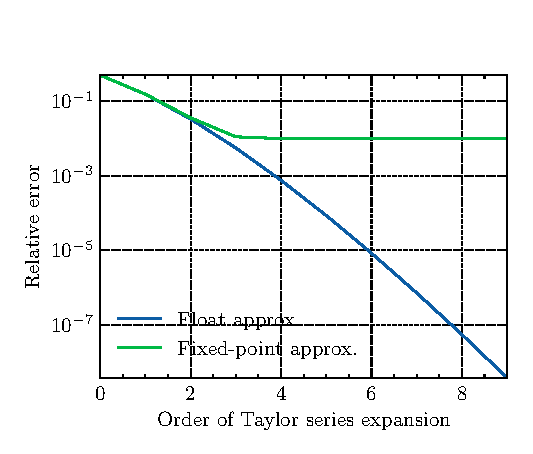
\includegraphics[width=0.9\textwidth]{assets/exp_approx_error.eps}
\end{figure}
\label{fig:exp_error}

\subsubsection{Square Root}
The square root module computes the square root of a fixed-point number using an iterative algortihm. It has a latency of $(N+Q)//2+1$ cycles, where $//$ denotes integer division. The module provides flags for overflow and 
negative radicand and start/busy/done signals. The module starts computation on an active-high pulse of the \texttt{start} signal and provides the result when the \texttt{done} signal is high.

\subsubsection{Multiply-Accumulate}
The \ac{mac} module performs a vector dot-product for a given pair of base addresses for the data and length of the vector and applies a selectable activation function to the result. Similar to the exponential module, it
uses shared adder, multiplier, divider and exponential modules in the \ac{cim} module. It can implement three activation functions: none, linear and Swish. For a nominal length of 64 (which corresponds to the embedding
depth of the model, a very common value for matrix dimensions in the model) and Q22.10 formate, the latencies are 386, 391 and 456, respectively. Note that, although the Swish activation function comprises a divider operation,
the \ac{mac} compute latency can still be kept fairly short because the divisor is the same for all elements. The module can thus perform the division once and multiply by the inverse, which is a single-cycle operation.Finally,
the \ac{mac} module can be directed to choose the second vector from weights or intermediate results memory.

\subsubsection{Softmax}
The softmax module computes the softmax function of a vector of fixed-point numbers. Similarly to the \ac{mac} module, it uses shared adder, mulitplier, divider and exponential modules and provides \texttt{busy} and
\texttt{done} signals. For a 64-element Q22.10 vector, the latency is 2024 cycles. This is significantly longer than other vector compute modules such as the \ac{mac} because, in the softmax operation, each element is exponantiated
individually.

\subsubsection{LayerNorm}
The final compute module is the LayerNorm module. It computes the Layer Normalization of a vector of fixed-point numbers. As described in section \ref{sec:vision_transformer}, the LayerNorm operation consists of a normalization of
the vector on the horizontal dimension followed by scaling and shifting using learnable parameters on the vertical dimension. Because each \ac{cim} module stores one vector at a time, the LayerNorm operation must be separated into 
two stages with a matrix transpose broadcast between the two. The latency for the first half is 1469 cycles and the latency for the second half is 494 cycles. The module provides \texttt{busy} and \texttt{done} signals and is controlled
with a \texttt{half-select} and \texttt{start} pulse signals. Because the length of the vector is constrained to be a power of two, the module uses bit-shifting instead of division for the normalization operation to decrease latency and energy
per operation.

\subsection{A Note About Software-Hardware Co-Design}

\lipsum[1]

\newpage
\section{Evaluation of Performance Metrics}
\lipsum[1]
\subsection{Vision Transformer}
\lipsum[1]
\subsection{Accelerator}
\lipsum[1]

\newpage
\section{Future Work}
\lipsum[1]

\newpage
\section{Conclusion}
\lipsum[1]

\newpage

% Bibliography
\printbibliography
\newpage

% Appendices
\appendix
\section{Codebase Statistics}
It may be interesting to the reader to appreciate the size of the codebase needed to develop a project of similar scale. The code for this project is available 
in my \href{https://github.com/TristanRobitaille/engsci-thesis}{GitHub repository}. The following table provides a breakdown of the number of lines of code in the project.

\begin{table}[ht]
    \centering
    \renewcommand{\arraystretch}{1.2} % Vertical spacing
    \setlength{\arrayrulewidth}{1.5pt} % Thickness of vertical lines
    \caption{Line and file count per file type in the codebase.}
    \begin{tabular}{@{} p{4cm}cccr @{}}
        \toprule
        File type       & File count    & Line count    & Percent of total & \\\midrule
        Python          & 12            & 3000          & 33.7\% \\
        SystemVerilog   & 12            & 2500          & 30.4\% \\
        C++             & 12            & 1250          & 18.9\% \\
        TeX             & 12            & 670           & 8.2\%  \\
        Shell           & 12            & 300           & 4.3\%  \\
        Other           & 12            & 20            & 4.5\%  \\\midrule
        Total           & 60            & 13,000         & 100\%  \\
        \hline
    \end{tabular}
    \label{tab:line_cnt}
\end{table}

In addition, there have been 200 commits to the repository.

\newpage
\section{Reflection on Learnings and Experience Gained}

% Flyleaf
\newpage
\thispagestyle{empty}
\vspace*{\fill}
\begin{center}
\Large
This page intentionally left blank.
\end{center}
\vspace*{\fill}

% Back cover
\newpage

\end{document}
